\clearpage
\appendix

\section{Statistics of KBs} \label{appendix:dataset}

\paragraph{\textbf{KBC Task.}} The statistics of KBs are shown in Table \ref{Statistics of the 50 KG for the two datasets} and Table \ref{Statistics of the 30 KG for the two datasets}. Note that isolated nodes refer to nodes that do not have any edges connecting to other nodes, and these nodes maintain self-loops (edges pointing to themselves). We retain those samples which have isolated entities (entities without any neighboring nodes). For the entity $e$ that is an isolated node, we add a triple, represented as $\langle e, noop, e \rangle$.
\renewcommand{\arraystretch}{1.2}
\begin{table}[h]
\centering
\setlength{\tabcolsep}{1pt}
\resizebox{0.45\textwidth}{!}{%
    \begin{tabular}{>{\centering\arraybackslash}p{1.4cm}>{\centering\arraybackslash}p{1.4cm}>{\centering\arraybackslash}p{1.4cm}>{\centering\arraybackslash}p{1.6cm}>{\centering\arraybackslash}p{1.4cm}>{\centering\arraybackslash}p{1.4cm}>{\centering\arraybackslash}p{2.3cm}}
    \toprule
    \textit{\textbf{Data set}} & \textit{\textbf{Entities}} & \textit{\textbf{Relations}} & \textit{\textbf{Train}} & \textit{\textbf{Valid}} & \textit{\textbf{Test}} & \textit{\textbf{Isolated nodes}} \\
    \midrule
    WebQSP     & 749,492 & 1,251 & 1,714,822 & 20,000 & 20,000 & 130,179 \\ 
    CWQ        & 672,970 & 1,232 & 1,479,924 & 20,000 & 20,000 & 119,654 \\ 
    \bottomrule
    \end{tabular}%
}
\caption{Statistics of the 50\% KB for the two data sets.}
\label{Statistics of the 50 KG for the two datasets}
\end{table}
\renewcommand{\arraystretch}{1}
\renewcommand{\arraystretch}{1.2}
\begin{table}[h]
\centering
\setlength{\tabcolsep}{1pt}
\resizebox{0.45\textwidth}{!}{%
\begin{tabular}{>{\centering\arraybackslash}p{1.4cm}>{\centering\arraybackslash}p{1.4cm}>{\centering\arraybackslash}p{1.4cm}>{\centering\arraybackslash}p{1.6cm}>{\centering\arraybackslash}p{1.4cm}>{\centering\arraybackslash}p{1.4cm}>{\centering\arraybackslash}p{2.3cm}}
    \toprule
    \textit{\textbf{Data set}} & \textit{\textbf{Entities}} & \textit{\textbf{Relations}} & \textit{\textbf{Train}} & \textit{\textbf{Valid}} & \textit{\textbf{Test}} & \textit{\textbf{Isolated nodes}} \\
    \midrule
    WebQSP  & 749,492 & 1,251 & 1,217,899 & 20,000 & 20,000 & 267,114 \\ 
    CWQ     & 672,970 & 1,232 & 1,060,601 & 20,000 & 20,000 & 244,439 \\ 
    \bottomrule
\end{tabular}%
}
\caption{Statistics of the 30\% KB for the two data sets.}
\label{Statistics of the 30 KG for the two datasets}
\end{table}
\renewcommand{\arraystretch}{1}

\paragraph{\textbf{KBQA Task.}} The statistics of the KBQA data sets used in this paper are shown in Table \ref{Statistics of KGQA datasets.}. Note that QA pairs in the training set without topic entities are removed. It can be seen that simply using the operation edge traverse on the complete KB could achieve nearly 100\% accuracy.
\renewcommand{\arraystretch}{1.2}
\begin{table}[h]
\centering
\setlength{\tabcolsep}{2.5pt}
\resizebox{0.45\textwidth}{!}{%
\begin{tabular}{>{\centering\arraybackslash}p{1.4cm}>{\centering\arraybackslash}p{2.5cm}>{\centering\arraybackslash}p{1.4cm}>{\centering\arraybackslash}p{1.4cm}>{\centering\arraybackslash}p{1.4cm}>{\centering\arraybackslash}p{2cm}}
\toprule
\textit{\textbf{Data set}} & \textit{\textbf{Answer format}} & \textit{\textbf{Train}} & \textit{\textbf{Test}} & \textit{\textbf{Coverage}} & \textit{\textbf{Licence}} \\
\midrule
WebQSP  & Entity/Number & 2777 & 3531 & 0.992 &  CC Licence \\ 
CWQ     & Entity & 23013 & 1639 & 0.997 & -\\ 
\bottomrule
\end{tabular}%
}
\caption{Statistics of KBQA data sets. Coverage refers to the accuracy of subgraph matching.}
\label{Statistics of KGQA datasets.}
\end{table}
\renewcommand{\arraystretch}{1}


\paragraph{\textbf{Reasoning Paths.}} The statistics of reasoning paths are shown in Table \ref{Statistics of Reasoning Paths}. In both KBQA data sets, the inference paths involve less than 1\% of the KBC test triples, indicating that even if the KBQA reasoning path is fully learned, its impact on the KBC test set remains minimal.
\renewcommand{\arraystretch}{1.2}
\begin{table}[h!]
\centering
\setlength{\tabcolsep}{1pt}
\resizebox{0.45\textwidth}{!}{%
    \begin{tabular}{>{\centering\arraybackslash}p{2cm}>{\centering\arraybackslash}p{2.5cm}>{\centering\arraybackslash}p{2.5cm}>{\centering\arraybackslash}p{3.5cm}}
    \toprule
    \textit{\textbf{Data set}} & \textit{\textbf{Number$_{path}$}} & \textit{\textbf{Number$_{test}$}} & \textit{\textbf{Number$_{test}$/Number$_{path}$}} \\
    \midrule
    WebQSP     & 8,623   & 27   & 0.31 \\
    CWQ        & 39,776  & 73   & 0.18 \\
    \bottomrule
    \end{tabular}%
}
\caption{Statistics of the reasoning path. \textit{\textbf{Number$_{path}$}} denotes the number of triples in the inference paths. \textit{\textbf{Number$_{test}$}} denotes the number of triples belonging to inference paths within the KBC test set.}
\label{Statistics of Reasoning Paths}
\end{table}
\renewcommand{\arraystretch}{1}


\section{Supplementary Experiment Settings} \label{appendix:settings}
\textbf{Evaluation Measures.} For KBC, we adopt the evaluation measures mean reciprocal rank (MRR) and Hits@$i$ ($i \in \{1, 3, 10\}$). MRR is calculated by averaging the reciprocal ranks of true tail entities over all test triples. Hits@$i$ evaluates the proportion of true tail entities in the top $i$ predictions. 
For KBQA, we adopt the evaluation measure Hits@1.(the proportion of true answers in the top $1$ predictions) to evaluate all methods. 

\noindent\textbf{KBC task.} For DIFT, we utilize SimKGC as the pre-trained KBC model. For IVR, we use ComplEx as the backbone. For BiNet, we utilize the BFS method to construct relational paths. 

\noindent\textbf{KBQA task.} For ToG and GoG, we change the prompt to adapt to Wikidata. For BiNet, we adopt the same setting as introduced above. 

% \renewcommand{\arraystretch}{1}
% \begin{table*}[th]
% \caption{Ablation study of the effect of the input sequence form of the SLM.}
% \centering
% \setlength{\tabcolsep}{2pt}
% \resizebox{\textwidth}{!}{
% \begin{tabular}{cccccccccccccccccccc}
% \toprule
% \multirow{2}{*}{\textit{\textbf{Task}}} 
% & \multirow{2}{*}{\textit{\textbf{Context}}} 
% & \textbf{\textit{Entity}} 
% & \textbf{\textit{Unified}}
% & \multicolumn{4}{c}{\textit{\textbf{WebQSP (30\%KB)}}} 
% & \multicolumn{4}{c}{\textit{\textbf{WebQSP (50\%KB)}}} 
% & \multicolumn{4}{c}{\textit{\textbf{CWQ (30\%KB)}}} 
% & \multicolumn{4}{c}{\textit{\textbf{CWQ (50\%KB)}}} \\ 
% \cmidrule(r){5-8} \cmidrule(r){9-12} \cmidrule(r){13-16} \cmidrule(l){17-20}

% & & \textit{\textbf{description}} & \textit{\textbf{question}} & \textit{MRR}   & \textit{Hits@1} & \textit{Hits@3} & \textit{Hits@10} & \textit{MRR}   & \textit{Hits@1} & \textit{Hits@3} & \textit{Hits@10} & \textit{MRR}   & \textit{Hits@1} & \textit{Hits@3} & \textit{Hits@10} & \textit{MRR}   & \textit{Hits@1} & \textit{Hits@3} & \textit{Hits@10} \\ 
% \cmidrule(r){1-20}
% \multirow{2}{*}{\textbf{KBC}}  &\Checkmark   & \Checkmark   & \Checkmark   & 0.601 & 0.570 & 0.624 & 0.656  & 0.631 & 0.601 & 0.654 & 0.684  & 0.580 & 0.550 & 0.603 & 0.635 & 0.631 & 0.601 & 0.653 & 0.683 \\ 
% & \XSolidBrush & \XSolidBrush & \XSolidBrush & 0.517 & 0.485 & 0.537 & 0.581  & 0.544 & 0.509 & 0.565 & 0.610  & 0.503 & 0.467 & 0.524 & 0.569 & 0.536 & 0.501 & 0.559 & 0.602 \\
% \midrule

% \multirow{2}{*}{\textbf{KBQA}}  &\Checkmark   & \Checkmark   & -   & - & 0.757 & - & -  & - & 0.759 & - & -  & - & 0.531 & - & - & - & 0.537 & - & - \\ 
% & \XSolidBrush & \XSolidBrush & -   & - & 0.731 & - & -  & - & 0.738 & - & -  & - & 0.517 & - & - & - & 0.520 & - & - \\
% \bottomrule
% \end{tabular}%
% }
% \label{Effect Analysis of the information for Joint Fine-Tuning T5}
% \end{table*}
% \renewcommand{\arraystretch}{1}

% \renewcommand{\arraystretch}{1.5}
% \begin{table*}[!t]
% \caption{Ablation study of the effect of the input sequence form of the SLM.}
% \centering
% \setlength{\tabcolsep}{1.2pt}
% \resizebox{\textwidth}{!}{
% \begin{tabular}{ccccccccccccccccccc}
% \toprule
% \multirow{2}{*}{\textbf{$\mathcal{T}$}} 
% & \multirow{2}{*}{\textit{\textbf{\makecell[c]{\textbf{$\mathcal{D}$}}}}} 
% & \multirow{2}{*}{\textit{\textbf{\makecell[c]{Query2question}}}}
% & \multicolumn{4}{c}{\textit{\textbf{WebQSP (30\% KB)}}} 
% & \multicolumn{4}{c}{\textit{\textbf{WebQSP (50\% KB)}}} 
% & \multicolumn{4}{c}{\textit{\textbf{CWQ (30\% KB)}}} 
% & \multicolumn{4}{c}{\textit{\textbf{CWQ (50\% KB)}}} \\ 
% \cmidrule(r){4-7} \cmidrule(r){8-11} \cmidrule(r){12-15} \cmidrule(l){16-19}

% &  &  
% & \textit{MRR}   & \textit{Hits@1} & \textit{Hits@3} & \textit{Hits@10} 
% & \textit{MRR}   & \textit{Hits@1} & \textit{Hits@3} & \textit{Hits@10} 
% & \textit{MRR}   & \textit{Hits@1} & \textit{Hits@3} & \textit{Hits@10} 
% & \textit{MRR}   & \textit{Hits@1} & \textit{Hits@3} & \textit{Hits@10} \\ 
% \cmidrule(r){1-19}

% \Checkmark   & \Checkmark   & \Checkmark   
%     & \textbf{0.593} & \textbf{0.562} & \textbf{0.616} & \textbf{0.649} 
%     & \textbf{0.624} & \textbf{0.594} & \textbf{0.645} & \textbf{0.681} 
%     & \textbf{0.584} & \textbf{0.552} & \textbf{0.607} & \textbf{0.640} 
%     & \textbf{0.609} & \textbf{0.578} & \textbf{0.631} & \textbf{0.662} \\ 

% \Checkmark   & \XSolidBrush   & \Checkmark 
% &0.566	&0.533	&0.583	&0.626
% &0.598	&0.565	&0.620	&0.657
% &0.530	&0.496	&0.552	&0.595
% &0.582	&0.548	&0.605	&0.643 \\

% \Checkmark   & \Checkmark   & \XSolidBrush 
% &0.588	&0.554	&0.607	&0.638
% &0.619	&0.586	&0.638	&0.672
% &0.579	&0.544	&0.603	&0.632
% &0.617	&0.582	&0.626	&0.659 \\

% \Checkmark   & \XSolidBrush   & \XSolidBrush
% &0.555	&0.522	&0.579	&0.619
% &0.595	&0.562	&0.618	&0.655
% &0.526	&0.490	&0.550	&0.593
% &0.569	&0.534	&0.593	&0.632 \\

% \XSolidBrush & \XSolidBrush & \XSolidBrush 
%     & 0.517 & 0.485 & 0.537 & 0.581    
%     & 0.544 & 0.509 & 0.565 & 0.610 
%     & 0.503 & 0.467 & 0.524 & 0.569  
%     & 0.536 & 0.501 & 0.559 & 0.602 \\
% \bottomrule
% \end{tabular}%
% }
% \label{Effect Analysis of the information for Joint Fine-Tuning T5}
% \end{table*}
% \renewcommand{\arraystretch}{1}

\renewcommand{\arraystretch}{1.3}
\begin{table*}[hbt]
\centering
\setlength{\tabcolsep}{1.2pt}
\resizebox{\textwidth}{!}{
\begin{tabular}{p{0.8cm}p{0.8cm}cccccccccccccccc}
\toprule
\multirow{2}{*}{\textbf{$\mathcal{T}$}} 
& \multirow{2}{*}{\textit{\textbf{\makecell[c]{\textbf{$\mathcal{D}$}}}}} 
& \multicolumn{4}{c}{\textit{\textbf{WebQSP (30\% KB)}}} 
& \multicolumn{4}{c}{\textit{\textbf{WebQSP (50\% KB)}}} 
& \multicolumn{4}{c}{\textit{\textbf{CWQ (30\% KB)}}} 
& \multicolumn{4}{c}{\textit{\textbf{CWQ (50\% KB)}}} \\ 
\cmidrule(r){3-6} \cmidrule(r){7-10} \cmidrule(r){11-14} \cmidrule(l){15-18}

& 
& \textit{MRR}   & \textit{Hits@1} & \textit{Hits@3} & \textit{Hits@10} 
& \textit{MRR}   & \textit{Hits@1} & \textit{Hits@3} & \textit{Hits@10} 
& \textit{MRR}   & \textit{Hits@1} & \textit{Hits@3} & \textit{Hits@10} 
& \textit{MRR}   & \textit{Hits@1} & \textit{Hits@3} & \textit{Hits@10} \\ 
\cmidrule(r){1-18}

\Checkmark   & \Checkmark
    & \textbf{0.603} & \textbf{0.572} & \textbf{0.628} & \textbf{0.652} 
    & \textbf{0.630} & \textbf{0.599} & \textbf{0.652} & \textbf{0.693} 
    & \textbf{0.588} & \textbf{0.556} & \textbf{0.612} & \textbf{0.645} 
    & \textbf{0.614} & \textbf{0.583} & \textbf{0.634} & \textbf{0.670} \\ 

\Checkmark   & \XSolidBrush
&0.566	&0.533	&0.583	&0.626
&0.598	&0.565	&0.620	&0.657
&0.530	&0.496	&0.552	&0.595
&0.582	&0.548	&0.605	&0.643 \\

\XSolidBrush & \Checkmark
    & 0.581 & 0.550 & 0.603 & 0.634    
    & 0.603 & 0.572 & 0.626 & 0.656   
    & 0.570 & 0.539 & 0.590 & 0.625  
    & 0.598 & 0.568 & 0.620 & 0.650   \\

\XSolidBrush & \XSolidBrush
    & 0.517 & 0.485 & 0.537 & 0.581    
    & 0.544 & 0.509 & 0.565 & 0.610 
    & 0.503 & 0.467 & 0.524 & 0.569  
    & 0.536 & 0.501 & 0.559 & 0.602 \\
\bottomrule
\end{tabular}%
}
\caption{Ablation study of the effect of the input sequence form of the SLM.}
\label{Effect Analysis of the information for Joint Fine-Tuning T5}
\end{table*}
\renewcommand{\arraystretch}{1}

\section{Baselines} \label{appendix:baseline}
\subsection{KBC Methods} \label{appendix:baseline:kbc}
For this task, we compare JCQL with eleven SOTA approaches as follows: 
\begin{itemize}[left=0pt]
\item TransE \cite{bordes2013} computes the candidate tail entity' score by representing relationships as vector translations.
\item DistMult \cite{yang2015} uses a bilinear scoring function with a diagonal relationship matrix to calculate scores of candidate tail entities.
\item ComplEx \cite{trouillon2016complex} extends DistMult by embedding entities and relations in a complex space.
\item RotatE \cite{sun2018rotate} obtains the score of tail entities by defining the relationship as rotations to capture a wider range of relational patterns.
\item IVR \cite{xiao2024knowledge} represents entities and relationships as embedding matrices and computes scores using a tensor decomposition model.
\item GoldE \cite{GoldE} computes the score of tail entities by applying hyperbolic orthogonal transformations to head entities and calculating the inner product with tail entities to capture hierarchical and geometric structures in knowledge graphs.

\item SimKGC \cite{wang-etal-2022-simkgc} leverages contrastive learning to optimize query embeddings derived from BERT, and computes the scores of candidate tail entities using the cosine similarity.
\item CSProm-KG \cite{chen-etal-2023-dipping} uses the embedding of entities and relationships to generate conditional soft prompts, which are then entered into the frozen SLM to predict the tail entity.
\item DIFT \cite{liu2024finetuninggenerativelargelanguage} predicts candidate tail entity by a pre-trained KBC model and refines the selection process with LLaMA.
\item SATKGC \cite{satkgc} proposes a subgraph-aware training framework that incorporates structural inductive biases into SLMs by utilizing random-walk based subgraph sampling as mini-batches and employing contrastive learning to prioritize topologically hard negatives based on shortest path distances.
\item RAA-KGC \cite{raa-kgc} proposes a relation-aware anchor enhancement strategy that utilizes neighbors of the head entity sharing the same relation as context.
\item BiNet \cite{lihui2022binet} converts multi-hop questions into relational paths via an encoder-decoder structure and utilizes a shared embedding space with an answer scoring module for joint optimization of KBC and KBQA.
\item KGT5 \cite{saxena2022kgt5} integrates KBC and KBQA tasks into a unified framework by converting the query and the question into a simple input sequence form and fine-tuning the model T5.
\end{itemize}

\begin{figure*}[t!]
    \centering
    \subfigure[]{
       \label{training_time:subfig:(a)}
        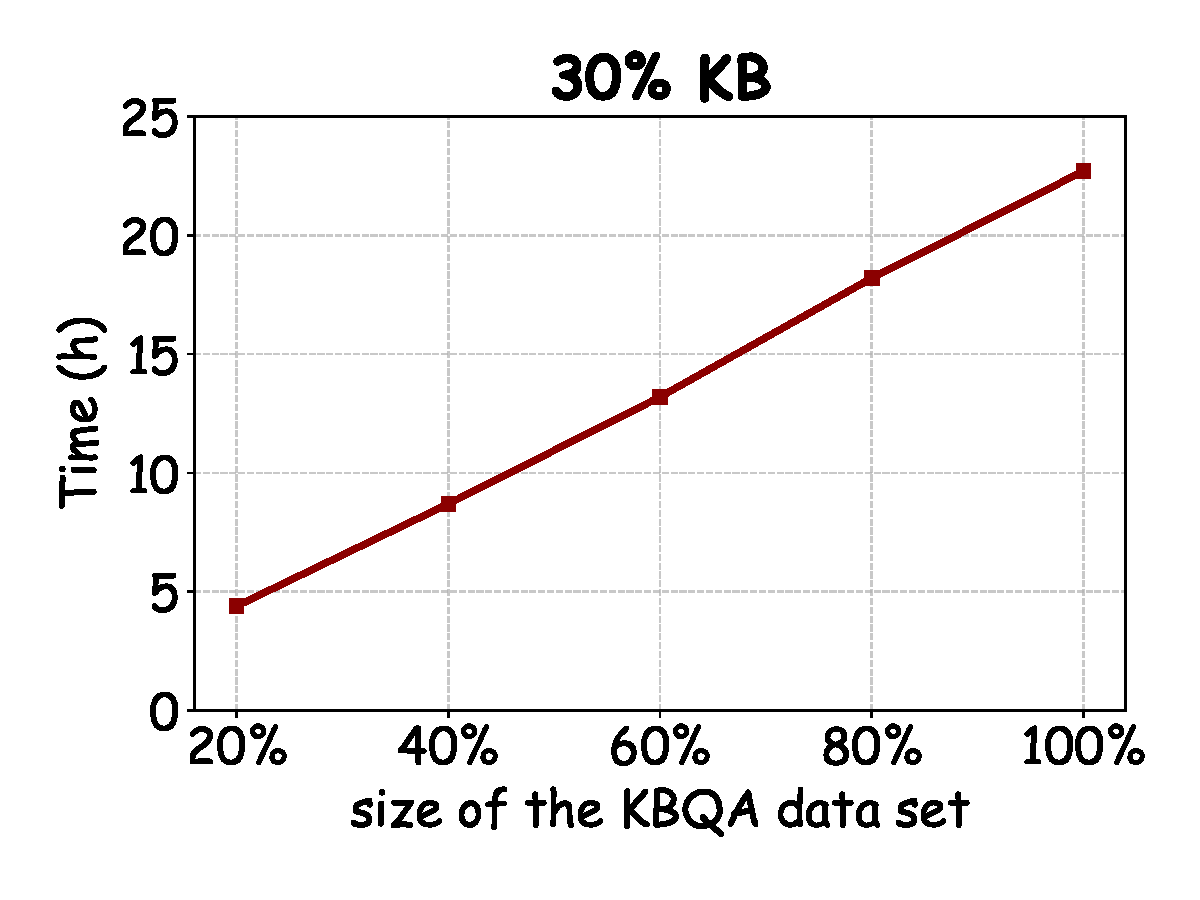
\includegraphics[width=0.4\textwidth]{image/img/training_time_30.pdf}}
    \subfigure[]{
       \label{training_time:subfig:(b)}
        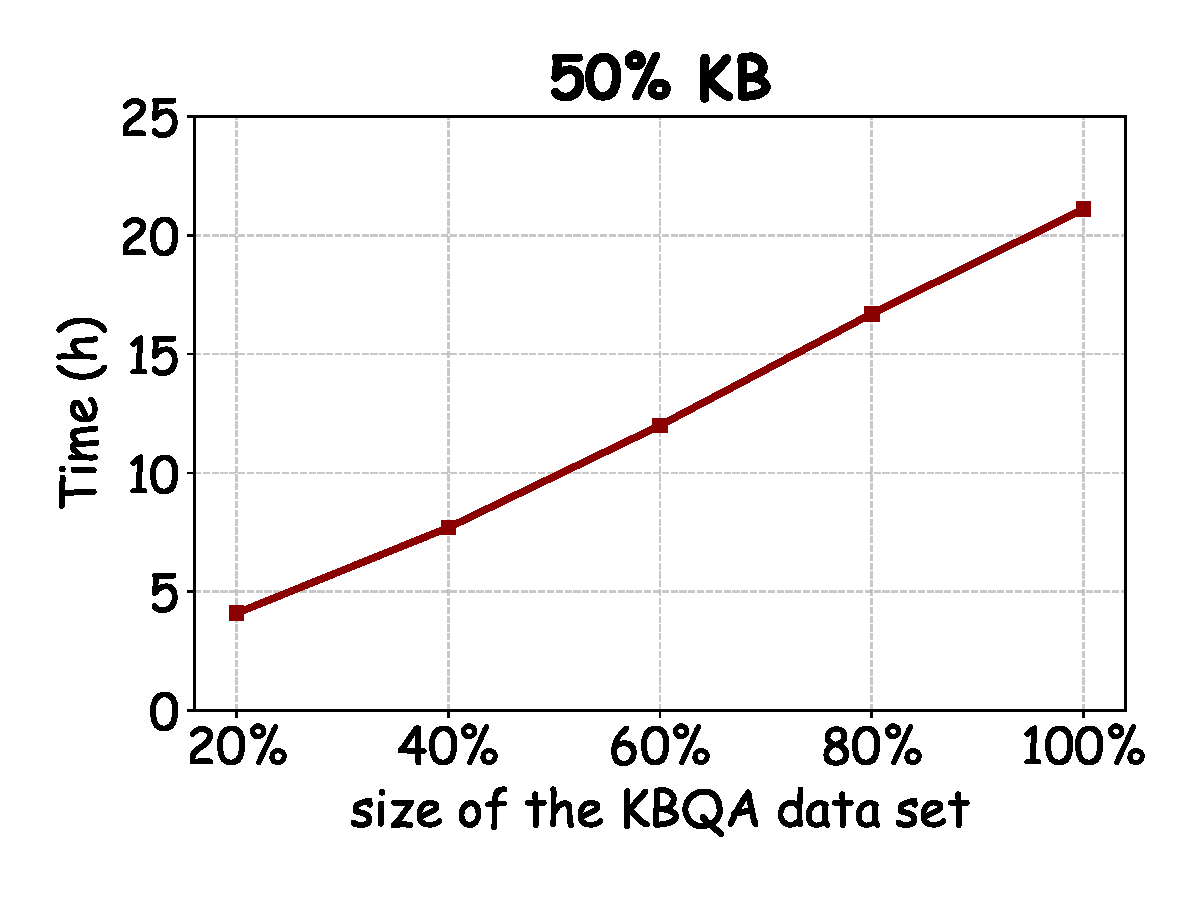
\includegraphics[width=0.4\textwidth]{image/img/training_time_50.pdf}}
    % \vspace{-3pt}
    \caption{Efficiency study of the training process on WebQSP.}
    \label{training time}
\end{figure*}
\begin{figure*}[t!]
  \centering
  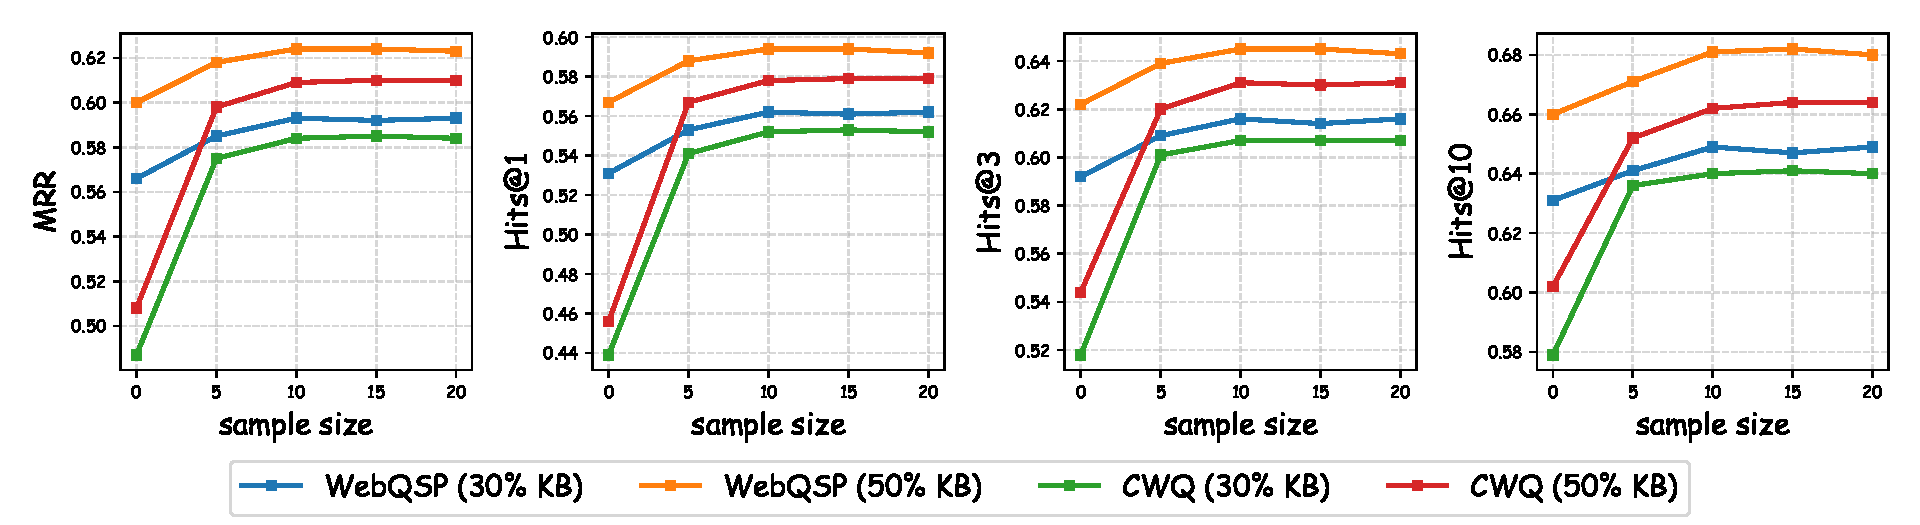
\includegraphics[width=0.95\linewidth]{image/img/sample_number_replay.pdf}
  \caption{Performance of JCQL with different sample numbers in experience replay.}
  \label{figure:Performance under Different Sample Numbers}
\end{figure*}

\subsection{KBQA Methods} \label{appendix:baseline:kbqa}
For this task, in addition to BiNet and KGT5, we use other baselines as follows:
\begin{itemize}[left=0pt]
\item GPT-4o-mini is adopted under the standard prompting\cite{brown2020languagemodelsfewshotlearners} without requiring the KB.
\item Chain-of-Thought (CoT) prompt \cite{wei2023chainofthoughtpromptingelicitsreasoning} solves questions through step-by-step reasoning without requiring the KB.
\item Self-Consistency (SC) \cite{wang2023selfconsistencyimproveschainthought} can generate multiple candidate answers via CoT and select the most consistent answer.
\item KG-CoT \cite{DBLP:conf/ijcai/Zhao0W0024} leverages a step-by-step graph reasoning model to perform reasoning over KBs and generates chains of knowledge with high confidence for LLMs based on the reasoning paths.
\item ToG \cite{sun2023thinkongraph} explores relation paths within KBs through iterative interactions with the LLM and let the LLM derive final answers based on the retrieved paths.
\item PoG \cite{Plan-on-Graph} adaptively explores and self-corrects reasoning paths to efficiently answer questions by leveraging guidance, memory, and reflection.
\item GoG \cite{xu-etal-2024-generate} retrieves triples from the KB and generates novel triples through the LLM to answer complex questions in the incomplete KB.
\item LMP \cite{lmp} adapts the message passing paradigm to the textual domain by iteratively condensing neighborhoods into hierarchical semantic facts, enabling LLMs to digest structural knowledge for effective reasoning.
\item PDRR \cite{pdrr} employs a semantic parsing-inspired framework to predict question types and decompose them into structured triples, enabling flexible planning for both chain and parallel reasoning over KGs.
\end{itemize}


\section{Supplementary Experimental Results} \label{appendix:supplementary_results}
% \subsection{Knowledge Base Completion} To gain deeper insight into the performance of JCQL in KBC, we conduct a comparative analysis of all baseline models with the Hits@10 metric. As shown in Table \ref{Knowledge Graph Completion Performance hits10}, JCQL also achieving the best performance in terms of Hits@10. % 为了进一步探究JCQL在KBC上的贡献，我们测试了所有baseline在Hits@10的性能。如图\ref{tables/KGC_compare_hits10}所示，JCQL在Hits@10上仍然达到了最佳性能。

\subsection{Effect Analysis of the Input Sequence Form of the SLM}
To verify the effectiveness of two kinds of information (i.e., entity description \textbf{$\mathcal{D}$} and context \textbf{$\mathcal{T}$}) introduced in Section \ref{sec:3.3}, we remove them from JCQL. As shown in Table \ref{Effect Analysis of the information for Joint Fine-Tuning T5}, without \textbf{$\mathcal{D}$} and \textbf{$\mathcal{T}$}, the performance of JCQL declines for KBC task on both data sets under different settings, which demonstrates the effectiveness of them. 

% \subsection{Effect Analysis of Different Numbers of Completed Triples}
% We investigate how the number of completed triples influence JCQL's performance. As depicted in Figure \ref{num_complete_triples}, JCQL performance generally improves with more triples, peaking before declining. This decline is likely due to the noise and irrelevant knowledge introduced by excessive complementation. Crucially, complementing the knowledge base with any number of predicted triples enhances the reasoning capacity for the KBQA task compared to the absence of complementation (i.e., $k=0$).

\subsection{Efficiency Study of Training Process}
In this subsection, we study the efficiency of JCQL's training process under different settings. Figure \ref{training_time:subfig:(a)} and Figure \ref{training_time:subfig:(b)} plot the total running time on WebQSP under different settings i.e., 30\% and 50\% of the KB, respectively. From the results, we can see that the total running time is approximately linear to the number of questions in the training data set, which is consistent with calls to the LLM described in Section \ref{sec:3.4}. Note that the running time of $\textsc{Parse}(C_q,\mathcal{M}_L)$ and $\textsc{IncFineTune}(\{\langle h,r,t\rangle\},P_q,\mathcal{M}_S)$ is negligible compared with $\textsc{Agent}(q,a_q,e_q,\mathcal{M}_S)$. Therefore, the training time mainly depends on $\textsc{Agent}(q,a_q,e_q,\mathcal{M}_S)$.

\subsection{Performance of JCQL with different sample size in experience replay.} To explore the influence of the sample size in experience replay on JCQL’s performance, we conduct experiments with the size set to $\{0, 5, 10, 15, 20\}$. As shown in Figure \ref{figure:Performance under Different Sample Numbers}, JCQL’s performance improves with the sample size. 
This suggests that our experience replay strategy can effectively mitigate catastrophic forgetting in SLM. It also demonstrates that performance growth diminishes when the sample size exceeds 10. To balance performance and computational cost, we set the sample size to 10.

% \begin{figure}[ht]
%     \centering
%     \includegraphics[width=0.75\linewidth]{image/img/num relevant triples in Complete Action.pdf}
%     \caption{Performance under different number of the completed triples}
%     \label{num_complete_triples}
% \end{figure}

% \begin{figure*}[t!]
%     \centering
%     \subfigure[WebQSP]{
%        \label{completed:subfig:(a)}
%         \includegraphics[width=0.35\textwidth]{image/img/num relevant triples in Complete Action left.pdf}}
%     \subfigure[CWQ]{
%        \label{completed:subfig:(b)}
%         \includegraphics[width=0.35\textwidth]{image/img/num relevant triples in Complete Action right.pdf}}
%     \vspace{-5pt}
%     \caption{Performance under different number of the completed triples}
%     \label{num_complete_triples}
% \end{figure*}

% \begin{figure*}[t!]
%     \centering
%     \includegraphics[width=1\linewidth]{image/img/num relevant triples in Complete Action.pdf}
%     \vspace{-9pt}
%     \caption{Performance under different number of completed triples.}
%     \label{num_complete_triples}
% \end{figure*}

\section{Prompt List} \label{appendix:prompt}
% \subsection{Prompts in Training Phase}\label{appendix:prompt:training phase}
% The following shows the prompts used in JCQL including Knowledge Extraction Prompt, KBQA Inference Selecting Entity and Template Consistency Prompt.

\subsection{Prompts for JCQL}\label{appendix:prompt:framework}
As shown in Prompt \ref{prompts for instruction used in knowledge extraction}, the prompt is designed to extract the reasoning process of KBQA. 
% \textcolor[rgb]{0,0.4392,0.7529}{The blue font} indicates the retrieved answers, \textcolor[rgb]{0.7529,0,0}{the red font} indicates \texttt{Generate Action} and \textcolor[rgb]{0.4549,0.7137,0.0078}{the green font} indicates \texttt{Complete Action}.
\begin{tcolorbox}[prompt=
{\begin{prompt} \label{prompts for instruction used in knowledge extraction}The Prompt for the Training Phase of JCQL 
\end{prompt}}]
$\bullet$ Instruction: \\ \\
Solve a question answering task with interleaving Thought, Action, Observation steps. Thought can reason about the current situation, and Action can be four types: \\
\textbf{(1) Search[entity1 | entity2 | ...],} which searches the exact entities on Wikidata and returns their one-hop subgraphs. You should extract all concrete entities appeared in your last thought without redundant words, and you should always select entities from topic entities in the first search. \\
\textbf{(2) Complete[head entity | relation],} which completes tail entities based on the head entity and relationships. \\ 
\textbf{(3) Generate[subquestion],} which generates some new triples related to your last thought. The subquestion should be a one-hop question. \\
\textbf{(4) Finish[answer1 | answer2 | ...],} which summarizes the answers from the triples and returns the true answers. You should reason about the answer based on the known triples. Firstly, you need to summarize all possible answers appeared in the known triples. Secondly, you should compare them with the reference answers. Finally, you should return all the true answers. If you don't know the answer, please return Finish[unknown].\\
You should generate each step without redundant words. \\

$\bullet$ Example: \\ \\
\textbf{Question:} where did woodrow wilson go to school? \\
\textbf{Topic Entity:} [Woodrow Wilson] \\
\textbf{Answer:} Davidson College | University of Virginia School of Law | Princeton University | Johns Hopkins University \\
\textbf{Thought 1:} The task requires identifying educational institutions attended by Woodrow Wilson. Based on the question, I will focus on gathering educational institutions linked to him. \\
\textbf{Action 1:} Search[Woodrow Wilson] \\
\textbf{Observation 1:} Woodrow Wilson, educated at, \textcolor[rgb]{0,0.4392,0.7529}{Davidson College} \\
Woodrow Wilson, employer, Bryn Mawr College \\
Woodrow Wilson, educated at, University of Virginia \\
\textbf{Thought 2:} While Davidson College and the University of Virginia are identified, I suspect there are more institutions. I will use the "Complete" action with "Woodrow Wilson" and the relation "educated at" to find additional schools. \\
\textbf{Action 2:} \textcolor[rgb]{0.4549,0.7137,0.0078}{Complete[Woodrow Wilson | educated at]} \\
\textbf{Observation 2:} Woodrow Wilson, educated at, \textcolor[rgb]{0,0.4392,0.7529}{Princeton University} \\
\textbf{Thought 3:} The result of Complete Action shows that Princeton University is also the school attended by Woodrow Wilson. I need to conduct further analysis to determine if there are other possible institutions. \\
\textbf{Action 3:} \textcolor[rgb]{0.7529,0,0}{Generate[which additional educational institutions are linked to Woodrow Wilson?]} \\
\textbf{Observation 3:} Woodrow Wilson, educated at, \textcolor[rgb]{0,0.4392,0.7529}{Johns Hopkins University} \\
\textbf{Thought 4:} Firstly, I have gathered four educational institutions associated with Woodrow Wilson: Davidson College, University of Virginia, Princeton University, and Johns Hopkins University. Secondly, I compare them completely with the reference answers. The University of Virginia School of Law is missing. \\
\textbf{Action 4:} Finish[Davidson College | University of Virginia | Princeton University | Johns Hopkins University] \\
\textbf{Observation 4:} Davidson College | Princeton University | Johns Hopkins University
\end{tcolorbox}
% \input{prompts/prompts for example used in knowledge extraction}

% \subsection{Prompts in Inference Phase}\label{appendix:prompt:inference phase}
As shown in Prompt \ref{prompts for instruction used in KGQA inference.}, the prompt is designed to executive reasoning for KBQA via the agent. \textcolor[rgb]{0,0.4392,0.7529}{The blue font} denotes the retrieved answers, \textcolor[rgb]{0.7529,0,0}{the red font} denotes the action \texttt{generate}, and \textcolor[rgb]{0.4549,0.7137,0.0078}{the green font} denotes the action \texttt{complete}.



\begin{tcolorbox}[prompt=
{\begin{prompt} \label{prompts for instruction used in KGQA inference.} The Prompt for the Inference Phase of JCQL
% Prompts for instruction used in the inference phase for KBQA task.
\end{prompt}}]

$\bullet$ Instruction: \\ \\
Solve a question answering task with interleaving Thought, Action, Observation steps. Thought can reason about the current situation, and Action can be four types:  \\
\textbf{(1) Search[entity1 | entity2 | ...],} which searches the exact entities on Wikidata and returns their one-hop subgraphs. You should extract all concrete entities appeared in your last thought without redundant words, and you should always select entities from topic entities in the first search.  \\
\textbf{(2) Complete[head entity | relation],} which completes tail entities based on the head entity and relationships. \\ 
\textbf{(3) Generate[subquestion],} which generates some new triples related to your last thought. The subquestion should be a one-hop question.  \\
\textbf{(4) Finish[answer1 | answer2 | ...],} which summarizes the answers based on all the known triples. You should reason about the answer based on the known triples. If you don't know the answer, please return Finish[unknown]. \\
You should generate each step without redundant words. \\

$\bullet$ Example: \\ \\
\textbf{Question:} Which one of Shakespeare's parents worked as a business person? \\
\textbf{Topic Entity:} [William Shakespeare] \\
\textbf{Thought 1:} I need to find Shakespeare's parents firstly. \\
\textbf{Action 1:} Search[William Shakespeare] \\
Observation 1: Judith Quiney, father, William Shakespeare \\
\textbf{Thought 2:} The search results did not provide specific information about William Shakespeare's parents or their occupations. Therefore, I need to identify Shakespeare's father. \\
\textbf{Action 2:} Generate[who are William Shakespeare's father?] \\
\textbf{Observation 2:} William Shakespeare, father, John Shakespeare \\
\textbf{Thought 3:} I could find the father of William Shakespeare is John Shakespeare. I need to identify Shakespeare's mother then. \\
\textbf{Action 3:} \textcolor[rgb]{0.7529,0,0}{Generate[who are William Shakespeare's mother?]} \\
Observation 3: William Shakespeare, mother, Mary Shakespeare \\
\textbf{Thought 4:} According to the generate results, I can find the father of William Shakespeare is John Shakespeare and the mother is Mary Shakespeare. So next I will search for some information about their occupations. \\
\textbf{Action 4:} Search[John Shakespeare | Mary Shakespeare] \\
\textbf{Observation 4:} John Shakespeare, child, Joan Shakespeare \\
Mary Shakespeare, spouse, John Shakespeare \\
Mary Shakespeare, occupation, writer \\
\textbf{Thought 5:} I find the occupation of Mary Shakespeare is writer, but the search results did not provide specific information about John Shakespeare's occupations. Therefore, I need to identify his business-related activities. \\
\textbf{Action 5:} \textcolor[rgb]{0.4549,0.7137,0.0078}{Complete[John Shakespeare | occupation]} \\
Observation 5: \textcolor[rgb]{0,0.4392,0.7529}{John Shakespeare}, occupation, merchant \\
John Shakespeare, occupation, politician \\
\textbf{Thought 6:} John Shakespeare is identified as William Shakespeare's father with occupations as a glove maker and a local government official. This connects him to the business realm. Therefore, I can summarize the answers. \\
\textbf{Action 6:} Finish[John Shakespeare]


\end{tcolorbox}


% \input{prompts/prompts for example used in KGQA inference}

\subsection{Supplementary Prompts for JCQL}\label{appendix:prompt:supplementary}
As shown in Prompt \ref{prompts for selecting entity}, the prompt is designed to select entities that are most related to the last \texttt{thought} based on the description of entities. During the reasoning, LLM may generate ambiguous entity names. With Prompt \ref{prompts for selecting entity}, LLM will select the suitable entity.
\begin{tcolorbox}[prompt=
{\begin{prompt} \label{prompts for selecting entity}The Prompt for Entity Selection
\end{prompt}}]
$\bullet$ Instruction: \\ \\
Given entities and their descriptions, please select the entity that is most related to the thought. \\ 
\\
$\bullet$ Example: \\ \\
\textbf{Thought: }Based on the given observation, I need to find out who the leader of America is. \\
\textbf{Entity Name: }Libya \\
\textbf{Candidate Entities:} \\
Q30: country primarily located in North America \\
Q106315054: vocal track by Donna Fargo; 1974 studio recording \\
Q99281400: country of the United States of America as depicted in Star Trek \\
\textbf{Answer: }Q30
\end{tcolorbox}

As shown in Prompt \ref{prompts for selecting relations}, the prompt is designed to select relations that are most related to the last \texttt{thought} in the action \texttt{search}.



\begin{tcolorbox}[prompt=
{\begin{prompt} \label{prompts for selecting relations}The Prompt for Relation Selection
\end{prompt}}]
$\bullet$ Instruction: \\ \\
Please select 3 relations that most relevant to the thought and rank them. \\ 
\\
$\bullet$ Example: \\ \\
\textbf{Thought: }The task requires identifying educational institutions attended by Woodrow Wilson.  I will focus on gathering educational institutions associated with him. \\
\textbf{Entity Name: }Woodrow Wilson \\
\textbf{Relations:} sibling, award received, signatory, owned by, doctoral student, spouse, member of, educated at, child, occupation, described by source, archives at, topic's main category, member of political party, place of burial, successful candidate, father, residence, employer, named after, work location, writing language, position held, sex or gender, candidate, given name, family name, candidacy in election\\
\textbf{Answers:} educated at, employer, named after
\end{tcolorbox}

As shown in Prompt \ref{prompts for generating triples}, the prompt is designed to generate new triples that are most related to the sub-question in the action \texttt{generate}. \textcolor[rgb]{0.98,0.4,0.5}{The pink font} indicates the supervision in the training phase of the KBQA task.


\begin{tcolorbox}[prompt=
{\begin{prompt} \label{prompts for generating triples}The Prompt for Triple Generation
\end{prompt}}]
$\bullet$ Instruction: \\ \\
Given the existing triples, please think step by step and generate new triples related to the current question. \\
\\
$\bullet$ Example: \\ \\
\textbf{Question:} what are the types of government in the United States? \\
\textcolor[rgb]{0.98,0.4,0.5}{\textbf{Hint:} federal republic | constitutional republic | presidential system} \\
\textbf{Known Triples: }""" \\
United States of America, instance of, country \\
United States of America, instance of, constitutional republic \\
United States of America, has cabinet, United States Cabinet \\
United States of America, basic form of government, republic \\
""" \\
\textbf{Generated Triples: }""" \\
1. United States of America, instance of, federal republic \\
2. United States of America, instance of, Democratic Republic \\
3. United States of America, basic form of government, presidential system \\
""" 
\end{tcolorbox}

\renewcommand{\arraystretch}{2.0}
\begin{table*}[t!]
\centering
\begin{tabular}{>{\hspace{0pt}}m{0.1\linewidth}|>{\hspace{0pt}}m{0.85\linewidth}} 
\hline
\rowcolor[rgb]{0.9490,0.9490,0.9490} 
\textbf{input} & $\langle$ Justin\ Bieber,\ father,\ ? $\rangle$ \\
\hline
\textbf{sequence} & predict tail: Justin Bieber $|$ father \par{} entity description: Justin Bieber [Canadian singer (born 1994)] \par{} related relationship: father \par{} context: $\langle$ Justin Bieber $|$ mother $|$ Pattie Mallette $\rangle$ $\langle SEP\rangle$ $\langle$ Justin Bieber $|$ sibling $|$ Jazmyn Bieber$\rangle$ $\langle SEP \rangle$ ... \\
\hline
\rowcolor[rgb]{0.9490,0.9490,0.9490} 
\textbf{output} & Jeremy Bieber \\
\hline
\end{tabular}
\caption{A typical case of input sequences and corresponding output for the SLM.}
\label{tab:cmp_kbc}
\end{table*}
\renewcommand{\arraystretch}{1}


We first link the relations within the generated triples to the canonical relations in the background KB using the BM25 algorithm. As shown in Prompt \ref{prompts for modifying triples}, the prompt is then designed to modify the triples generated by LLM. The LLM often frequently generates unreliable triples. For instance, this prompt may allow the LLM invert head-tail entity pairs, such as modifying $\langle$Pak Pong-ju, head of government, North Korea$\rangle$ into $\langle$North Korea, head of government, Pak Pong-ju$\rangle$. Specifically, as a pre-processing step, for each relation in the background KB, the description and schema are obtained by retrieving the original description from Wikidata and extracting multiple corresponding triples from the background KB. Subsequently, the original description and these triples are input into the LLM to generate refined description and to summarize the schema from the triples.


\begin{tcolorbox}[prompt=
{\begin{prompt} \label{prompts for modifying triples}The Prompt for Triple Modification
\end{prompt}}]
$\bullet$ Instruction: \\ \\
Please modify the known triples based on the descriptions and schemas of the relations. You should generate triples without redundant words. \\
\\
$\bullet$ Example: \\ \\
\textbf{Question: }who is ruling north korea now? \\
\textbf{Known Triples: }""" \\
North Korea, office held by head of state, Kim Il-sung \\
North Korea, office held by head of state, Kim Jong-un \\
Pak Pong-ju, head of government, North Korea \\
""" \\
\textbf{Descriptions: }""" \\
1. office held by head of state: This relation links a geographical or political entity... \\
2. member of political party: This relation connects individuals to the political parties... \\
3. head of government: This relation links a specific location—such as a city, municipality... \\
4. head of state: This relation links a geographical entity, such as a country or state... \\
""" \\
\textbf{Schemas: }""" \\
1. office held by head of state: [Location], office held by head of state, [Political Office] \\
2. member of political party: [Human], member of political party, [Political Party] \\
3. head of government: [Location], head of government, [Human] \\
4. head of state: [Location], head of state, [Human] \\
""" \\
\textbf{New Triples: }""" \\
1. North Korea, head of state, Kim Il-sung \\
2. North Korea, head of state, Kim Jong-un \\
3. North Korea, head of government, Pak Pong-ju \\
"""
\end{tcolorbox}

As shown in Prompt \ref{prompts for generating paths}, the prompt is designed to select the triples most relevant to the question to construct reasoning paths. 


\begin{tcolorbox}[prompt=
{\begin{prompt} \label{prompts for generating paths}The Prompt for Path Generation
\end{prompt}}]
$\bullet$ Instruction: \\ \\
Considering the known triples and relations, please select the triples and relations that are relevant to the questions and answers. \\
\\
$\bullet$ Example: \\ \\
\textbf{Question:} which one of Shakespeare's parents worked as a business person? \\
\textbf{Answer:} John Shakespeare \\
\textbf{Topic entity:} William Shakespeare \\
\textbf{Known triples:} """ \\
William Shakespeare, field of work, acting \\
William Shakespeare, field of work, poetry \\
William Shakespeare, field of work, theatre \\
William Shakespeare, father, John Shakespeare \\
William Shakespeare, mother, Mary Shakespeare \\
Mary Shakespeare, spouse, John Shakespeare \\
Mary Shakespeare, occupation, writer \\
John Shakespeare, occupation, merchant \\
John Shakespeare, occupation, politician \\
""" \\
\textbf{Related relations:} father, mother, occupation \\
\textbf{Related triples:} """ \\
William Shakespeare, father, John Shakespeare \\
William Shakespeare, mother, Mary Shakespeare \\
Mary Shakespeare, occupation, writer \\
John Shakespeare, occupation, merchant \\
John Shakespeare, occupation, politician \\
""" 
\end{tcolorbox}

% \section{Pseudocodes}
% The pseudocodes of JCQL are listed below.
% \begin{algorithm}[bth]
% \caption{KBQA Training}\label{alg:kgqa}
% \KwData{incomplete knowledge graph $G=\{E,R,T\}$, \texttt{question} $q$, \texttt{gold answers} $E_a$, hyper parameter $k$, max length of LLMs output $L$}
% \KwResult{\texttt{Top-k candidates}}
% $W=\{w_1,w_2 \dots, w_{|L|}\} \gets \texttt{Knowledge\_Extraction}(q, E_a)$\;
% $G_{q} \gets \texttt{construct\_subgraph}(W)$\;
% \For{\texttt{each} $e_a \in E_a$}{
% $\texttt{Path}\ P \gets \texttt{BFS}(e_t,e_a)$\;
% $\texttt{content}\ T_{c} \gets \texttt{Filter}(P)$\;
% $\texttt{Sequence}\gets$ \texttt{Concatenate topic entity }$e_a$, \texttt{entity description}, \texttt{relations in} $T_c$ and \texttt{context} $T_c$\;
% \texttt{Top-k candidates} $\gets \texttt{T5}(\texttt{Sequence})$\;
% }
% \end{algorithm}

% \begin{algorithm}[bth]
% \caption{KBC Training}\label{alg:kgc}
% \KwData{incomplete knowledge graph $G=\{E,R,T\}$, \texttt{training triples} $T=\{(h,r,t)\}$, \texttt{generated triples} $T_{gen}$, hyper parameter $k$}
% \KwResult{\texttt{Top-k candidates}}
% $T_{all} \gets T\ \cap\ T_{gen}$\;
% \For{\texttt{each} $(h,r,t) \in T_{all}$}{
% $\texttt{content}\ T_{c} \gets \texttt{Sample\_Neighbor}(h)$\;
% $\texttt{Sequence}\gets$ \texttt{Concatenate head entity }$h$, \texttt{entity description}, \texttt{relation} $r$ and \texttt{context} $T_c$\;
% \texttt{Top-k candidates} $\gets \texttt{T5}(\texttt{Sequence})$\;
% }
% \end{algorithm}

% \section{Notations and definitions} \label{appendix:notations and definitions}
% Table \ref{Notations and definitions.} gives the main notations used throughout this paper.

\section{Case Study} \label{appendix:case study}
% \paragraph{\textbf{Comparison between GoG and JCQL under 50\% KB.}}
\paragraph{\textbf{Comparison between \texttt{generate} and \texttt{complete} under 50\% KB.}}
JCQL treats LLM as both agent and KB, generating new triples from the internal knowledge of the LLM. However, when triples are missing, action \texttt{generate} over-relies on the LLM's internal knowledge, increasing the risk of hallucination. To alleviate this issue, our approach incorporates the SLM, ensuring that predicted relations and entities are assigned unique IDs. As shown in Table \ref{tab:cmp_gog}, action \texttt{generate} incorrectly generates relationships and entities that do not exist in the KB. In contrast, JCQL generates valid entities through its action \texttt{complete}.
\paragraph{\textbf{A typical case of input sequences and corresponding output for the SLM.}} table \ref{tab:cmp_kbc} shows a typical case of input sequences and corresponding output for the SLM. Given the query $\langle Justin\ Bieber, f ather, ? \rangle$, JCQL obtains triples with the one-hop neighborhoods of the head entity $Justin\ Bieber$ uniformly, at random and without replacement. Finally, we concatenate them with $\langle SEP \rangle$.

\renewcommand{\arraystretch}{1.5}
\begin{table*}[t!]
\centering
\begin{tabular}{>{\hspace{0pt}}m{0.1\linewidth}|>{\hspace{0pt}}m{0.83\linewidth}} 
\hline
\rowcolor[rgb]{0.8588,0.8588,0.8588} Question   & what type of government did soviet union have? \\ 
\hline
\rowcolor[rgb]{0.9490,0.9490,0.9490} JCQL w/o \texttt{complete}   & Thought 1:~I need to find out what type of government the Soviet Union had.\par{}Action 1:~Search[Soviet Union]\par{}Observation 1:~soviet union, history of topic, history of the soviet union\par{}soviet union, legislative body, supreme soviet of the soviet union\par{}soviet union, official religion, state atheism\par\null\par{}Thought 2:~The Soviet Union had a legislative body called the Supreme Soviet, which implies a type of government. I need to generate more information about the government structure of the Soviet Union based on this observation.\par{}Action 2:~\textcolor[rgb]{0.7529,0,0}{Generate[type of government of the Soviet Union]}\par{}Observation 2: soviet union, ideological basis, Marxism-Leninism\par{}soviet union, type of government, one-party socialist republic\par\null\par{}Thought 3:~The Soviet Union is characterized as a one-party socialist republic based on its ideological basis of Marxism-Leninism.\par{}Action 3:~Finish[one-party socialist republic]  \\
\hline
\rowcolor[rgb]{0.9490,0.9490,0.9490} JCQL w/o \texttt{generate}                     & Thought 1:~The question requires identifying the type of government in the Soviet Union. I should gather information regarding the political structure and governance of the Soviet Union.\par{}Action 1:~Search[Soviet Union]\par{}Observation 1:~Soviet Union, foundational text, Declaration of the Creation of the Union of Soviet Socialist Republics\par{}Soviet Union, foundational text, Treaty on the Creation of the Union of Soviet Socialist Republics\par{}Soviet Union, legislative body, Supreme Soviet of the Soviet Union\par{}member of the Supreme Soviet of the Russian Soviet Federative Socialist Republic, country, Soviet Union\par\null\par{}Thought 2:~The current information provides some context about the Soviet Union but lacks specific details about its type of government. I need to find the governance structure of the Soviet Union.\par{}Action 2:~\textcolor[rgb]{0.4549,0.7137,0.0078}{Complete[Soviet Union | instance of]}\par{}Observation 2: Soviet Union, instance of, country\par{}Soviet Union, instance of, \textcolor[rgb]{0,0.4392,0.7529}{socialist state}\par\null\par{}Thought 3:~The results indicate that the Soviet Union was a socialist state. This clarifies the type of government. Therefore, I can summarize the answers.\par{}Action 3:~Finish[\textcolor[rgb]{0,0.4392,0.7529}{socialist state}]. \\
\hline
\end{tabular}
\caption{The comparison between \texttt{generate} and \texttt{complete} under the setting i.e., 50\% KB.}
\label{tab:cmp_gog}
\end{table*}
\renewcommand{\arraystretch}{1}



% \section{Supplementary Related Work} 

\section{Supplementary Setting Details} \label{appendix:implementation_details}
In all experiments, the depth of exploration is set to $10$ to avoid endless exploration. The maximum token length for generation is set to $512$. All experiments are conducted on a server with an Intel(R) Xeon(R) Silver $4310$ CPU ($2.10$GHz), $256$ GB RAM memory, and an NVIDIA RTX A6000 GPU.

\section{Broader Impact} \label{appendix:limitations}
By performing KBQA and KBC jointly, JCQL enhances the complex reasoning abilities of the KB-augmented LLM and improves the performance of the SLM when faced with incomplete KBs. Furthermore, other broader impacts of JCQL are listed as follows. (1) The proposed framework JCQL is flexible. For KBQA, we can choose any KBC model to complete missing triples for any KB. 
(2) JCQL can generate reasoning paths based on input questions and update the KB in real time using incremental learning techniques, demonstrating its real-time performance and the ability of lifelong learning.
(3) From a long-term perspective, the LLM's reasoning paths generated from continuous increasing of question-answer pairs strengthen the KBC model, which in turn improves the reasoning capability of LLM.
